\documentclass[a4]{seminar}

\usepackage{palatino,epsfig}

\def\N{\mathsf{l\kern -.15em N}}
\def\Z{\mathsf{Z\kern -.4em Z}}
\def\Q{\mathsf{l\kern -.35em Q}}
\def\eqdef{\mathrel{\smash{\mathop{\kern 0pt{=}}\limits^{\hbox{\tiny def}}}}}
\def\depij{\mathrel{\smash{\mathop{\kern 0pt{\longrightarrow}}\limits^{\theta_i^j,\omega_i^j}}}}
\newtheorem{claim}{Claim}
\newtheorem{lemma}{Lemma}
\newtheorem{theorem}{Theorem}
\newtheorem{property}{Property}
\newtheorem{corollary}{Corollary}
\newtheorem{definition}{Definition}
\def\proof{\par\noindent{\em Proof: }}
\def\endproof{\ \hfill\lower 1ex\vbox{\hrule\hbox{\vrule\phantom
    p\vrule}\hrule}\medskip}

\usepackage{slidesec}

\newslideframe{IMAGE}{%
  \boxput{\rput(1,0){\includegraphics[scale=0.4]{st}}}{#1}}
\slideframe*{IMAGE}

\usepackage{pstcol} % To use the standard `color' package with Seminar
\usepackage{semcolor}
\usepackage{slidesec}
\input{seminar.bug}
\input{seminar.bg2} % See the Seminar bugs list

\usepackage{graphicx}
\usepackage{fancybox}

\usepackage{fancyhdr}
% Headers and footers personalization using the `fancyhdr' package
\fancyhf{} % Clear all fields
\renewcommand{\headrulewidth}{0.2mm}
\renewcommand{\footrulewidth}{0.2mm}
\fancyhead[L]{\small\textsf{A Machine Description System}}
\fancyhead[R]{\small\textsf{\theslideheading}}
%\fancyfoot[L]{\tiny\textsf\thedate}
\fancyfoot[L]{\scriptsize\textsf{April 12, 2005}}
\fancyfoot[R]{\scriptsize\textsf\theslide}
% To avoid that the headers be too close of the top of the page
\renewcommand{\slidetopmargin}{2cm}
% To center horizontally the headers and footers (see seminar.bug)
\renewcommand{\headwidth}{\textwidth}
% To adjust the frame length to the header and footer ones
\autoslidemarginstrue

\slideframe{none}

\begin{document}

\thispagestyle{empty}

\begin{slide}

\begin{center}

{\large\bf A Machine Description System \\
for Embedded Compilation Tools}

\vspace{15 mm}

{Beno\^{\i}t Dupont de Dinechin \\
%AST Embedded Systems Research Laboratory \\
%Via Cantonale 16E 6928 Manno Switzerland \\
\texttt{Benoit.Dupont-de-Dinechin@st.com}}

\vspace{5 mm}


\epsfig{file=EPS/stlogo.eps,width=20mm} {STMicroelectronics}

{\small April 12, 2005}

\end{center}

\end{slide}


\pagestyle{fancy}


\begin{slide}

\slideheading{Why a Machine Description System}

\begin{center} \underline{Software Development Tools Program Representations}
\end{center}

\begin{itemize}

\item Binary absolute and relocatable form

\item Assembler source and disassembler output

\item Assembler internal representation (instructions \& operands)

\item Compiler internal representation (operations \& parameters)

\end{itemize}

\begin{center} \underline{Software Development Tools ISA Representations}
\end{center}

\begin{itemize}

\item Binary encoding (operand, instructions, bundles)

\item Storage elements (memory, registers, constant generators)

\item Instruction behavior (instruction set simulation)

\item Instruction properties (compiler code optimizations)

\item Instruction semantics (compiler code selection)

\end{itemize}

\end{slide}


\begin{slide}

\begin{center} \underline{Purpose of a Machine Description System}
\end{center}

A Machine Description System (MDS) is a structured data repository and a
collection of programs used to configure the target-specific parts of the
software development tools.

\begin{center} \underline{Existing Machine Description Systems}
\end{center}

\begin{description}

\item[Green Hills Software] Canonical Machine Description to configure the
compiler, assembler, linker, disassembler, debugger.

\item[CMG Bristol Architects] CHESS tables to drive the documentation and the
instruction set simulator of the ST200 processors.

\item[Coware / LisaTek] Lisa language to automatically produce
simulators (instruction and cycle accurate), assembler, linker, debugger,
compiler instruction scheduler.

\end{description}

\end{slide}


\begin{slide}

\begin{description}

\item[U. of Virginia] Computer Systems Description Languages (CSDL). Different
languages and tools are available: SLED for encoding / decoding; RTL and
$\lambda$-RTL for instruction semantics; Alpha for calling conventions; Block
language for stack frame composition.

\item[Open64 TargInfo] Calls to a special C++ library to generate the Open64
target description tables and enumerations. This covers assembly syntax,
instruction encoding, bundling, scheduling, register allocation, ABI targeting.

\item[AST MachGen] C code \& data to configure the LxISS, the GNU AS, and to
generate constant evaluators for the LxBE.

\item[STS ARC \& CSD] Machine descriptions systems respectively used by the LAO
ST100 and the LAO ST200. The ARC covered assembly syntax, instruction encoding,
bundling, scheduling, register allocation, instruction properties and semantics.

\end{description}

\end{slide}


\begin{slide}

\begin{center} \underline{Lessons from these Machine Description Systems}
\end{center}

\begin{itemize}

\item The CSDL system from U. of Virginia is the most advanced, but is now a
disparate collection of language and tools.

\item The single language-based approaches (GHS, Lisa) mix the different
description levels and constrain the description into some hierarchy. A single
language cannot cover everything.

\item The authoring of machine descriptions in C++ (Open64 TargInfo, AST MachGen)
tends to be tool-centric so they do not include the descriptions they don't use.

\item Not able to describe aliases between storage locations (Open64).

\item No instruction selection / peephole re-selection generators.

\item No understanding of instruction bundling / bundle templates.

\item Not able to distinguish between core-specific and target-specific.

\end{itemize}

\end{slide}


\begin{slide}

\slideheading{The STMicroelectronics MDS}

\begin{center} \underline{Current Capabilities} \end{center}

\begin{itemize}

\item Production use for STMicroelectronics ST200 family, STMicroelectronics
STXP70 family, ARMv5e, ARMV6

\item High-speed instruction encoders and decoders for the STMicroelectronics JIT

\item Generation of the target-specific parts of the Open64, GNU AS

\end{itemize}

\begin{center} \underline{Short-Term Extensions} \end{center}

\begin{itemize}

\item Description of the ST40/SH4 and the STMicroelectronics XPE

\item Generation of the target-specific parts of GNU LD (PIC mode)

\item Stack frame building and ABI conventions with Stage Allocation.

\end{itemize}

\end{slide}


\begin{slide}

\begin{center} \underline{AST/STS MDS Organization and Flows} \end{center}

\begin{itemize}

\item Available under \texttt{http://mds.codex.cro.st.com/}

{\scriptsize
\begin{verbatim}
svn co https://svn.mds.codex.cro.st.com/svnroot/mds/trunk/MDS
mkdir build && cd build
../MDS/configure --target=st200 --with-cores="st240" --enable-tools="gnu o64"
make clean all check diff
\end{verbatim}
}

\item Front-end scripting creates the Machine Description Database (MDD) XML
tables from a variety of non-XML sources (CHESS, MachGen, special scripts)

\item The MDD XML tables are expanded using target-independent scripts into
Machine Description Expanded (MDE) XML tables; then the target-level
tables are merged across the different cores

\item Back-end scripting processes the MDS (MDD+MDE) XML tables and produce the
files needed by software development tools:  GNU AS tables, Open64 TargInfo, LAO
machine description, etc.

\end{itemize}

\end{slide}


\begin{slide}

\begin{center}
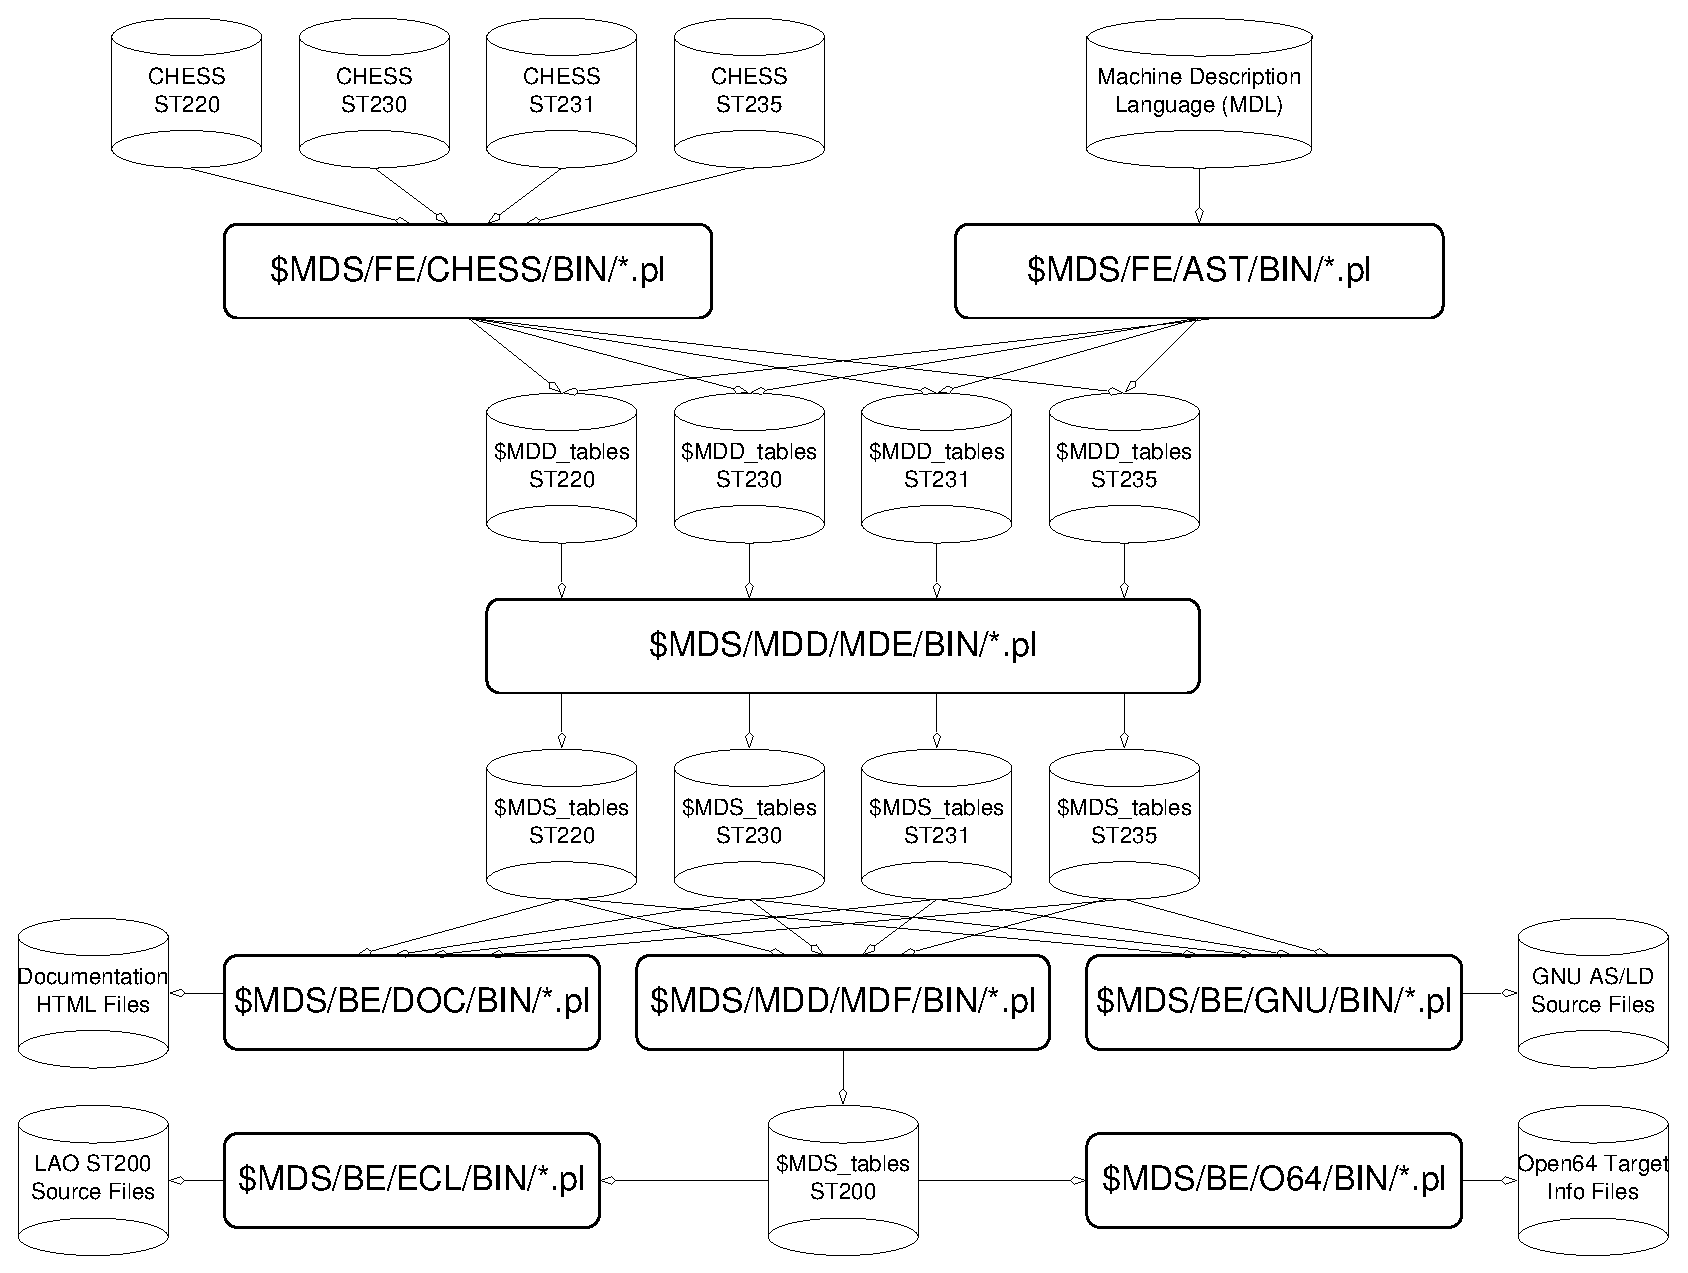
\epsfig{file=FIG/mds-flow.eps,width=100mm}
\end{center}

\end{slide}


\begin{slide}

\slideheading{Conclusions}

\begin{itemize}

\item The MDS has already accumulated several man-years of effort

\item The MDS as been used for two years for the STMicroelectronics production
compiler tools

\item Need to expand the MDS front-end with a 'pseudo-C' behavior language

\item Need to develop the extraction of semantic properties using tree pattern
matching techniques (prototyped)

\item Need to derive automatic SSA-based instruction selection and peephole
generation

\item More processors to de described

\end{itemize}

These objectives will be achieved withing the Sceptre project.

\end{slide}


\end{document}

